\documentclass[tikz,border=5mm]{standalone}
\usetikzlibrary{backgrounds,fit,shapes}

\begin{document}
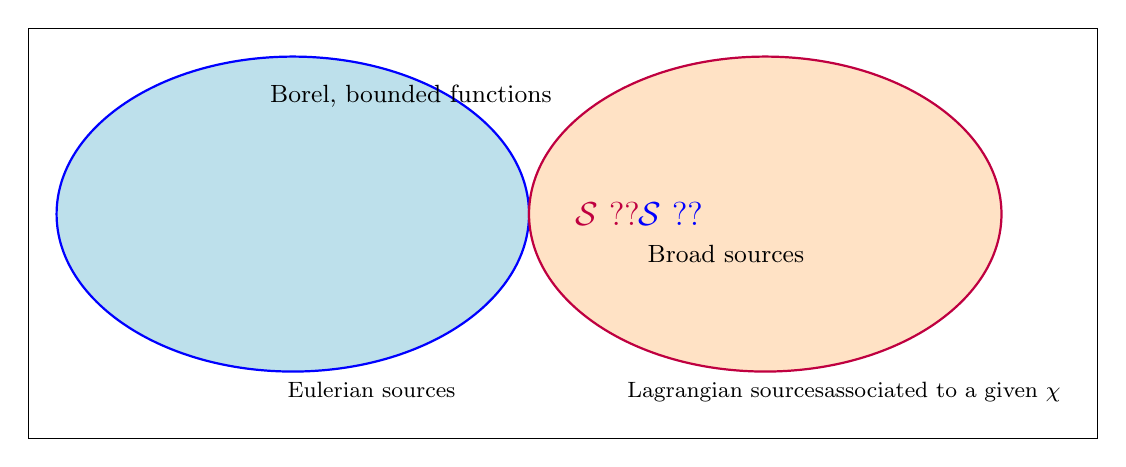
\begin{tikzpicture}[thick]
    % Define colors
    \definecolor{eulerian}{RGB}{173,216,230} % Light blue for Eulerian sources
    \definecolor{lagrangian}{RGB}{255,219,183} % Light orange for Lagrangian sources

    % Draw the Eulerian region
    \filldraw[eulerian!80, draw=blue] 
        (-4,0) ellipse (3cm and 2cm);

    % Draw the Lagrangian region
    \filldraw[lagrangian!80, draw=purple] 
        (2,0) ellipse (3cm and 2cm);

    % Draw the intersection area (light purple)
    \begin{scope}[on background layer]
        \clip (-4,0) ellipse (3cm and 2cm);
        \fill[white, opacity=0.5] (2,0) ellipse (3cm and 2cm);
    \end{scope}

    % Labels
    \node at (-2.5,1.5) [text width=4cm, align=center, font=\small] {Borel, bounded functions};
    \node at (-3,-2) [below, font=\footnotesize] {Eulerian sources};
    \node at (3,-2) [below, font=\footnotesize] {Lagrangian sources\\ associated to a given $\chi$};

    % Text in the intersection
    \node at (0,0) [font=\large] {\textcolor{purple}{$\mathcal S\ ??$}};
    \node at (0.8,0) [font=\large] {\textcolor{blue}{$\mathcal S\ ??$}};
    
    % Ellipse labels in the intersection
    \node at (1.5,-0.5) [font=\small] {Broad sources};

    % Outer bounding box
    \node[draw, inner sep=10pt, fit=(current bounding box), ultra thin] {};
\end{tikzpicture}
\end{document}